\chapter{Réalisation et implémentation}

\section{Introduction}

Ce chapitre présente la réalisation technique de la plateforme Virtual FabLab. Contrairement au chapitre précédent, qui décrit l’analyse et la conception, cette partie se concentre sur l’implémentation effective du projet : organisation du code, architecture frontend/backend, modules fonctionnels, simulation 3D, communication MQTT et tableau de bord de supervision.

La plateforme réalisée repose sur un backend FastAPI, une interface Next.js et des modules spécialisés pour la visualisation 3D, l’interprétation des fichiers de fabrication et l’analyse des données de télémétrie. Les données utilisées dans cette version sont simulées afin de valider l’architecture, les flux MQTT, le monitoring et le module d’analyse. La plateforme reste conçue pour être connectée ultérieurement à des capteurs réels.

\section{Architecture frontend/backend}

L’implémentation adopte une architecture séparant clairement le frontend et le backend. Le frontend prend en charge l’interface utilisateur, la navigation, les scènes 3D et les tableaux de bord. Le backend fournit les API, la sécurité, la base de données, l’ingestion MQTT et les traitements analytiques.

\begin{figure}[H]
\centering
\IfFileExists{images/implementation_architecture.png}
{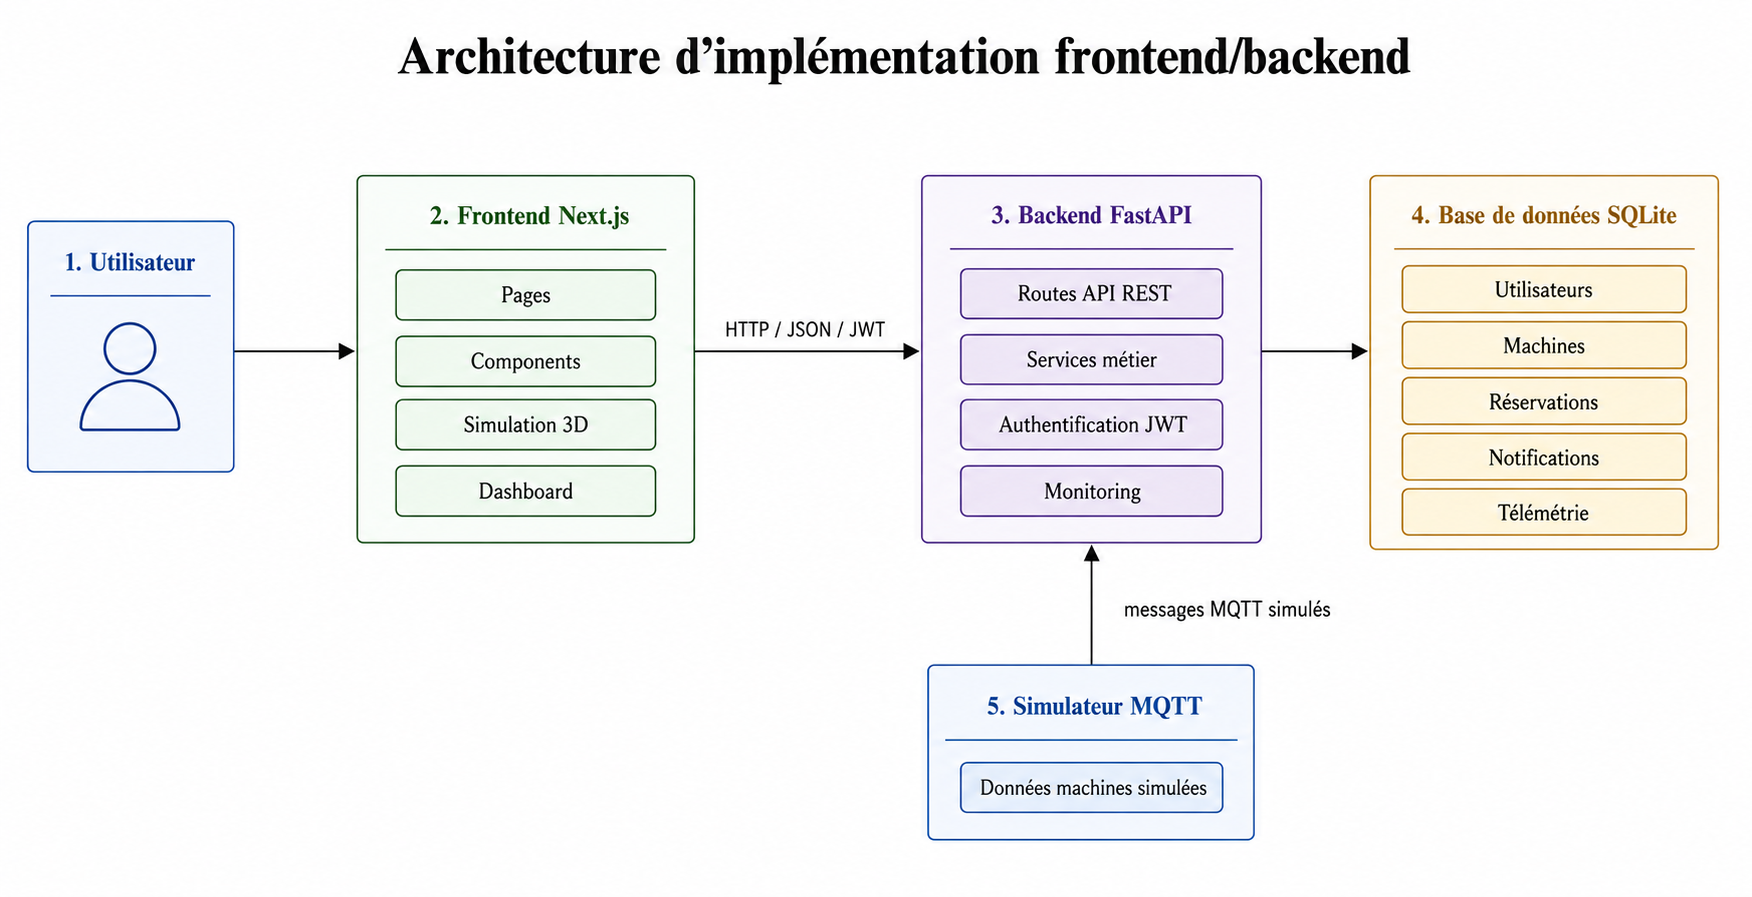
\includegraphics[width=0.95\textwidth]{images/implementation_architecture.png}}
{\fbox{\parbox[c][5.5cm][c]{0.85\textwidth}{\centering Emplacement réservé pour l’architecture d’implémentation\\\texttt{images/implementation\_architecture.png}}}}
\caption{Architecture d’implémentation frontend/backend}
\label{fig:implementation-architecture}
\end{figure}

Le backend est initialisé dans le point d’entrée FastAPI. Au démarrage, il initialise la base de données et lance le service abonné MQTT. Les routes sont ensuite organisées par domaine fonctionnel : authentification, machines, réservations, administration, monitoring, simulation, notifications et intelligence artificielle.

\section{Organisation des dossiers}

Le projet est organisé en trois parties principales : le frontend, le backend et le rapport LaTeX. Cette organisation facilite la maintenance et permet d’isoler les responsabilités.

\begin{table}[H]
\centering
\small
\caption{Organisation générale du projet}
\label{tab:organisation-projet}
\begin{tabular}{|p{0.28\textwidth}|p{0.62\textwidth}|}
\hline
\rowcolor{SectionColor!12}
\textbf{Dossier} & \textbf{Rôle} \\
\hline
\texttt{Frontend/app} & Pages principales de l’application Next.js : accueil, lab 3D, simulation, dashboard, réservations, utilisateurs et profil. \\
\hline
\texttt{Frontend/components} & Composants réutilisables : layout, authentification, scène 3D, simulation, tableaux de bord et composants UI. \\
\hline
\texttt{Frontend/lib} & Fonctions utilitaires, appels API, traductions et moteur d’interprétation des fichiers G-code/NC. \\
\hline
\texttt{backend/app/routes} & Définition des endpoints FastAPI par domaine fonctionnel. \\
\hline
\texttt{backend/app/services} & Logique métier : authentification, machines, réservations, télémétrie, MQTT, anomalies et prédiction. \\
\hline
\texttt{backend/app/models} & Modèles SQLModel représentant les entités persistées. \\
\hline
\texttt{backend/scripts} & Scripts de simulation MQTT et d’entraînement des modèles de Machine Learning. \\
\hline
\texttt{Rapport\_PFE} & Sources LaTeX du rapport académique. \\
\hline
\end{tabular}
\end{table}

\section{Implémentation du backend}

\subsection{API FastAPI}

Le backend expose une API REST structurée autour de plusieurs routeurs. Chaque routeur regroupe les endpoints liés à un domaine précis. Cette organisation améliore la lisibilité du code et facilite l’évolution de la plateforme.

Les principales familles d’endpoints sont :

\begin{itemize}
    \item \texttt{/auth} pour l’inscription, la connexion et le profil ;
    \item \texttt{/machines} pour la gestion administrative des machines ;
    \item \texttt{/lab/machines} pour l’affichage public des machines du FabLab ;
    \item \texttt{/reservations} pour les demandes de réservation ;
    \item \texttt{/admin} pour la gestion des utilisateurs et des réservations ;
    \item \texttt{/monitoring} pour la télémétrie et l’état MQTT ;
    \item \texttt{/simulation} pour l’état de simulation ;
    \item \texttt{/admin/ai} pour les analyses intelligentes réservées à l’administrateur.
\end{itemize}

\subsection{Base de données}

La persistance est assurée par SQLite avec SQLModel. Les modèles principaux sont les utilisateurs, les types de machines, les machines, les réservations, les mesures capteurs et les notifications.

\begin{figure}[H]
\centering
\IfFileExists{images/database_schema.png}
{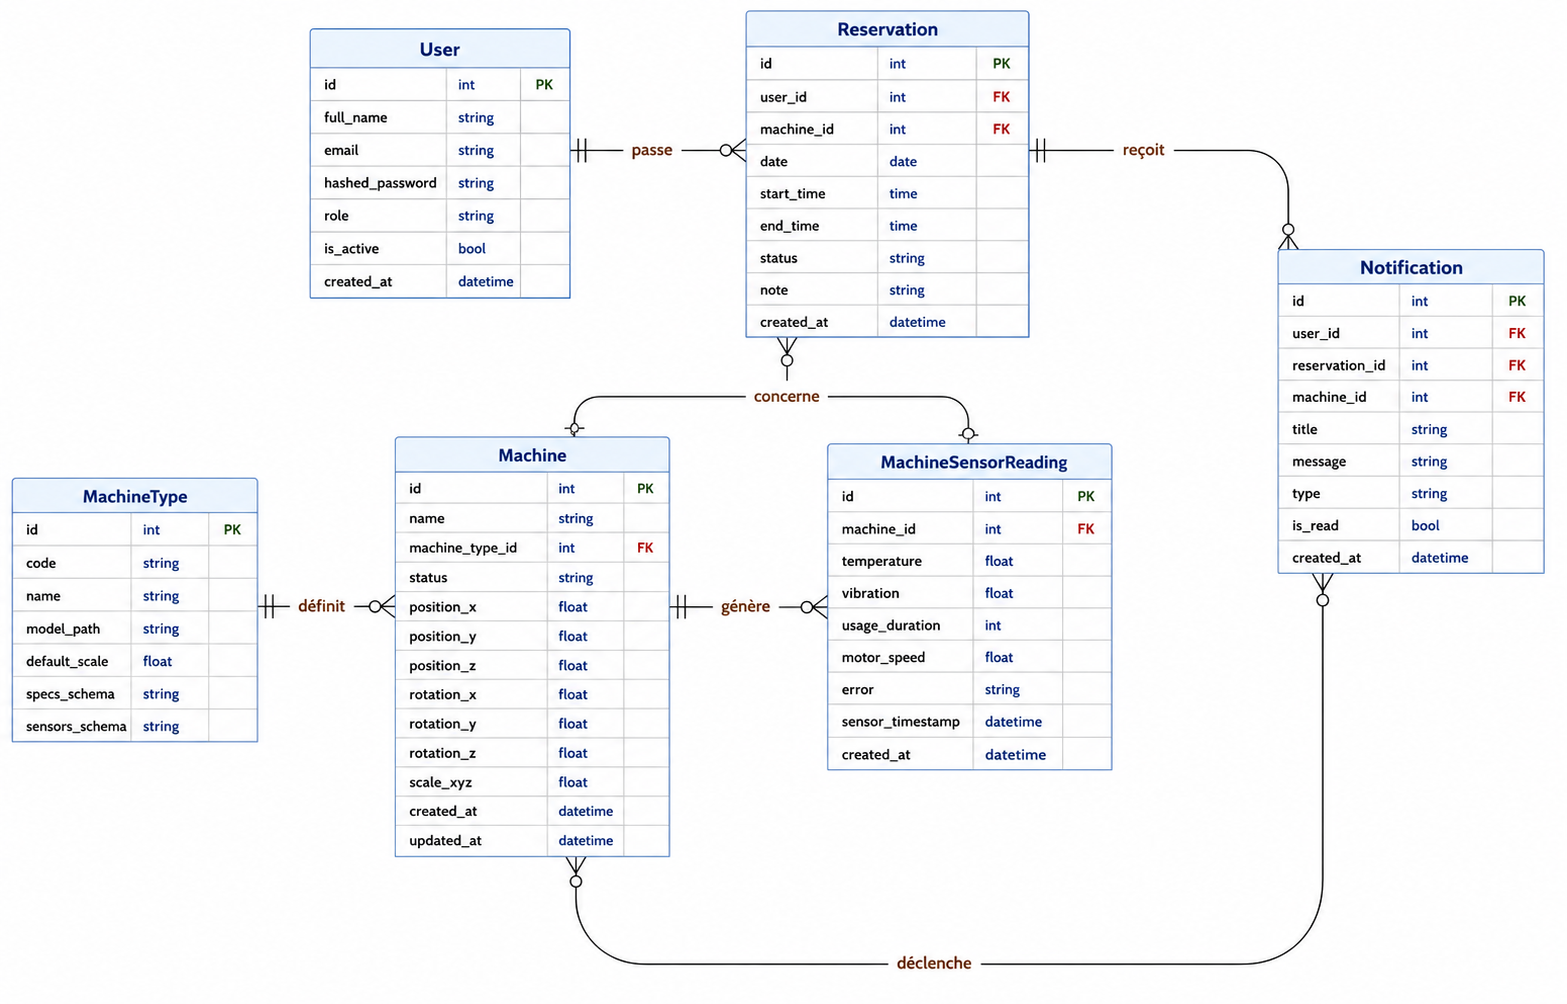
\includegraphics[width=0.95\textwidth,height=0.65\textheight,keepaspectratio]{images/database_schema.png}}
{\fbox{\parbox[c][5cm][c]{0.85\textwidth}{\centering Emplacement réservé pour le schéma de la base de données\\\texttt{images/database\_schema.png}}}}
\caption{Schéma logique de la base de données}
\label{fig:database-schema}
\end{figure}

\section{Système d’authentification}

L’authentification est basée sur des jetons JWT. Lorsqu’un utilisateur se connecte, le backend vérifie son email et son mot de passe haché, puis génère un jeton d’accès. Le frontend conserve ce jeton et l’ajoute dans l’en-tête \texttt{Authorization} lors des appels aux routes protégées.

Deux rôles sont définis dans le système :

\begin{itemize}
    \item \texttt{student} : rôle par défaut pour les utilisateurs inscrits ;
    \item \texttt{admin} : rôle permettant l’accès aux interfaces et endpoints d’administration.
\end{itemize}

\section{Gestion des utilisateurs et de l’administration}

L’espace administrateur permet de consulter les utilisateurs, de rechercher un compte, de filtrer par rôle ou par état, puis de modifier les droits. L’administrateur peut également activer ou désactiver un compte.

\begin{figure}[H]
\centering
\IfFileExists{images/screenshot_users_admin.png}
{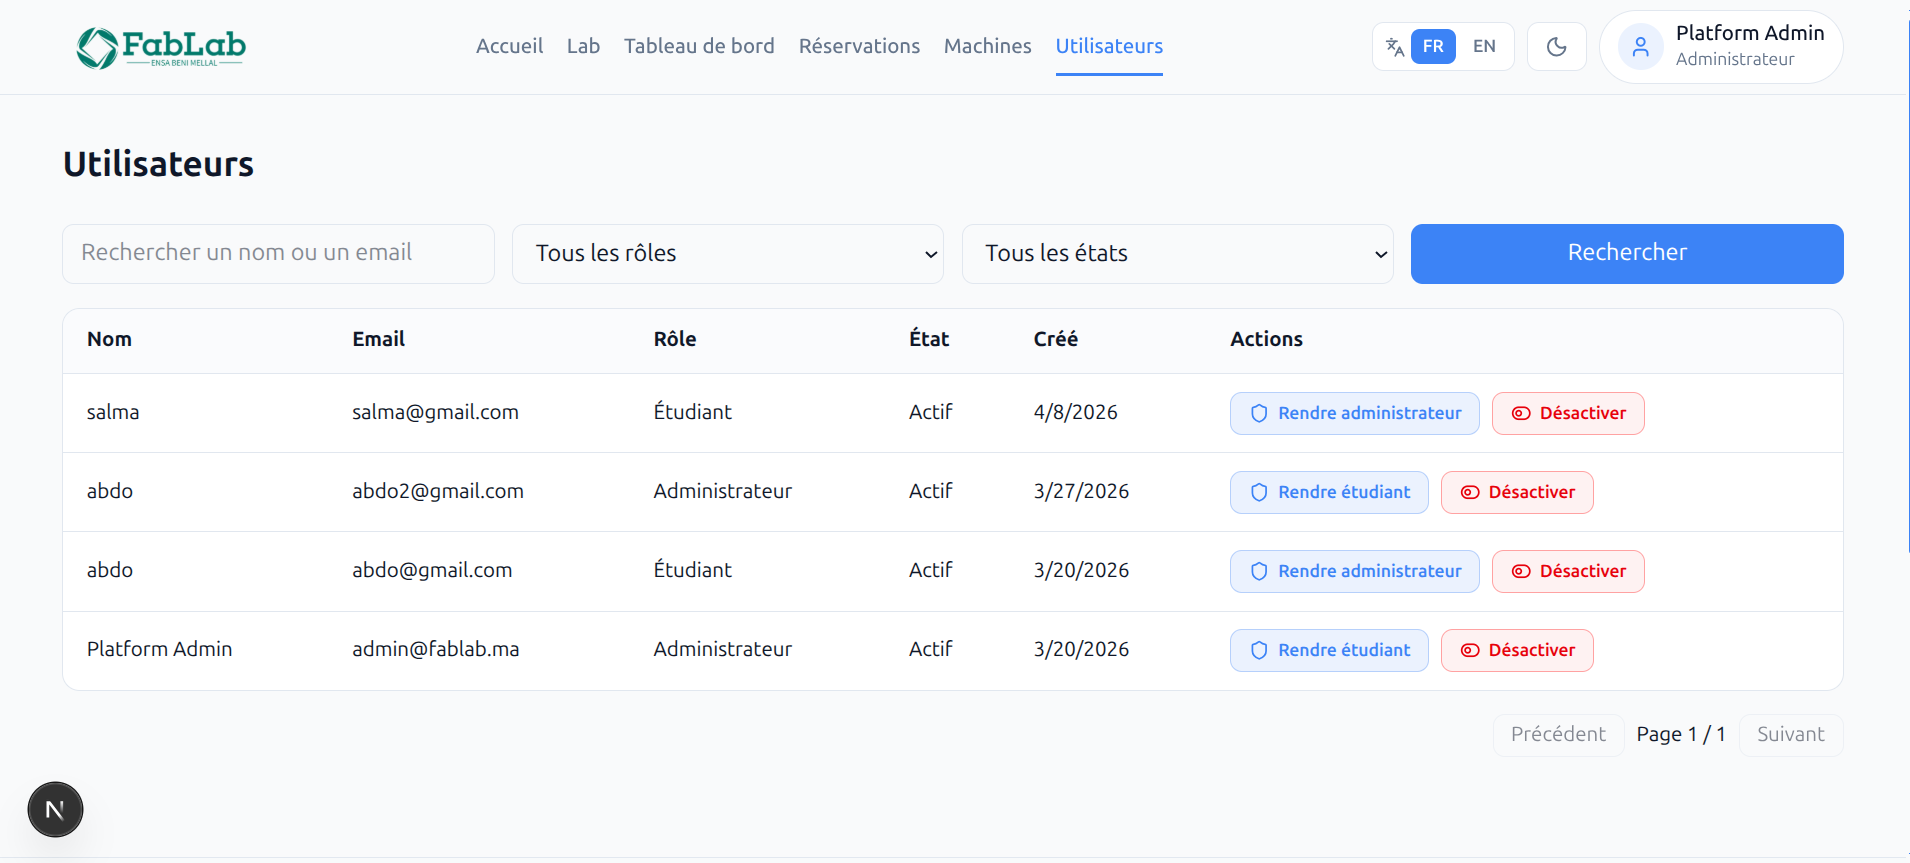
\includegraphics[width=0.95\textwidth]{images/screenshot_users_admin.png}}
{\fbox{\parbox[c][5cm][c]{0.85\textwidth}{\centering Emplacement réservé pour la gestion des utilisateurs\\\texttt{images/screenshot\_users\_admin.png}}}}
\caption{Interface de gestion des utilisateurs}
\label{fig:screenshot-users-admin}
\end{figure}

L’accès à ces fonctionnalités est protégé par une dépendance backend qui vérifie que l’utilisateur courant possède le rôle administrateur.

\section{Gestion des machines}

Le module machines permet de gérer les instances du FabLab. Chaque machine possède un type, un nom, un état, des notes et des paramètres de placement dans la scène 3D : position, rotation et échelle.

Les types de machines initialisés par défaut incluent notamment :

\begin{itemize}
    \item une imprimante 3D associée au modèle \texttt{/models/3d\_printer.glb} ;
    \item une machine CNC associée au modèle \texttt{/models/CNC.glb} ;
\end{itemize}

\begin{figure}[H]
\centering
\IfFileExists{images/screenshot_machines_admin.png}
{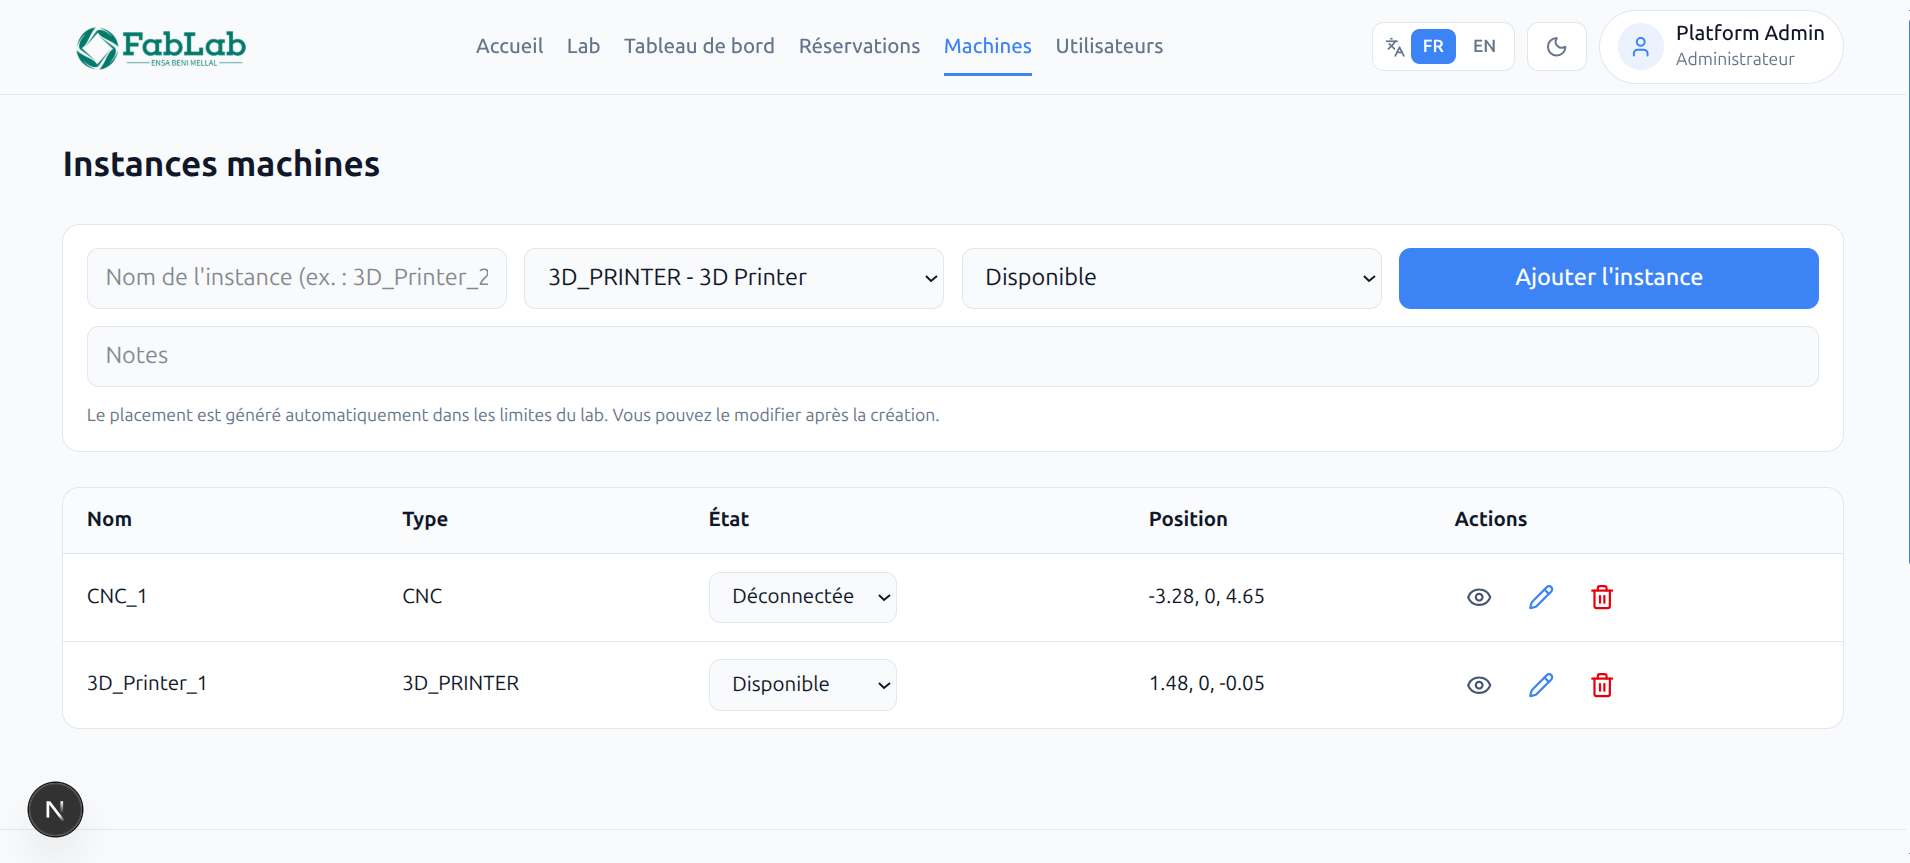
\includegraphics[width=0.95\textwidth]{images/screenshot_machines_admin.png}}
{\fbox{\parbox[c][5cm][c]{0.85\textwidth}{\centering Emplacement réservé pour l’interface de gestion des machines\\\texttt{images/screenshot\_machines\_admin.png}}}}
\caption{Interface de gestion des machines}
\label{fig:screenshot-machines-admin}
\end{figure}

\section{Système de réservation}

Le système de réservation permet à l’étudiant de choisir une machine, une date et un créneau horaire. Les créneaux sont générés entre 8h00 et 20h00 avec une durée d’une heure. Le backend vérifie les conflits afin d’empêcher deux réservations actives sur la même machine et le même intervalle.

Une demande de réservation est créée avec l’état \texttt{pending}. L’administrateur peut ensuite approuver ou refuser cette demande. Lorsqu’une décision est prise, une notification est créée pour l’utilisateur concerné.

\begin{figure}[H]
\centering
\IfFileExists{images/screenshot_reservations.png}
{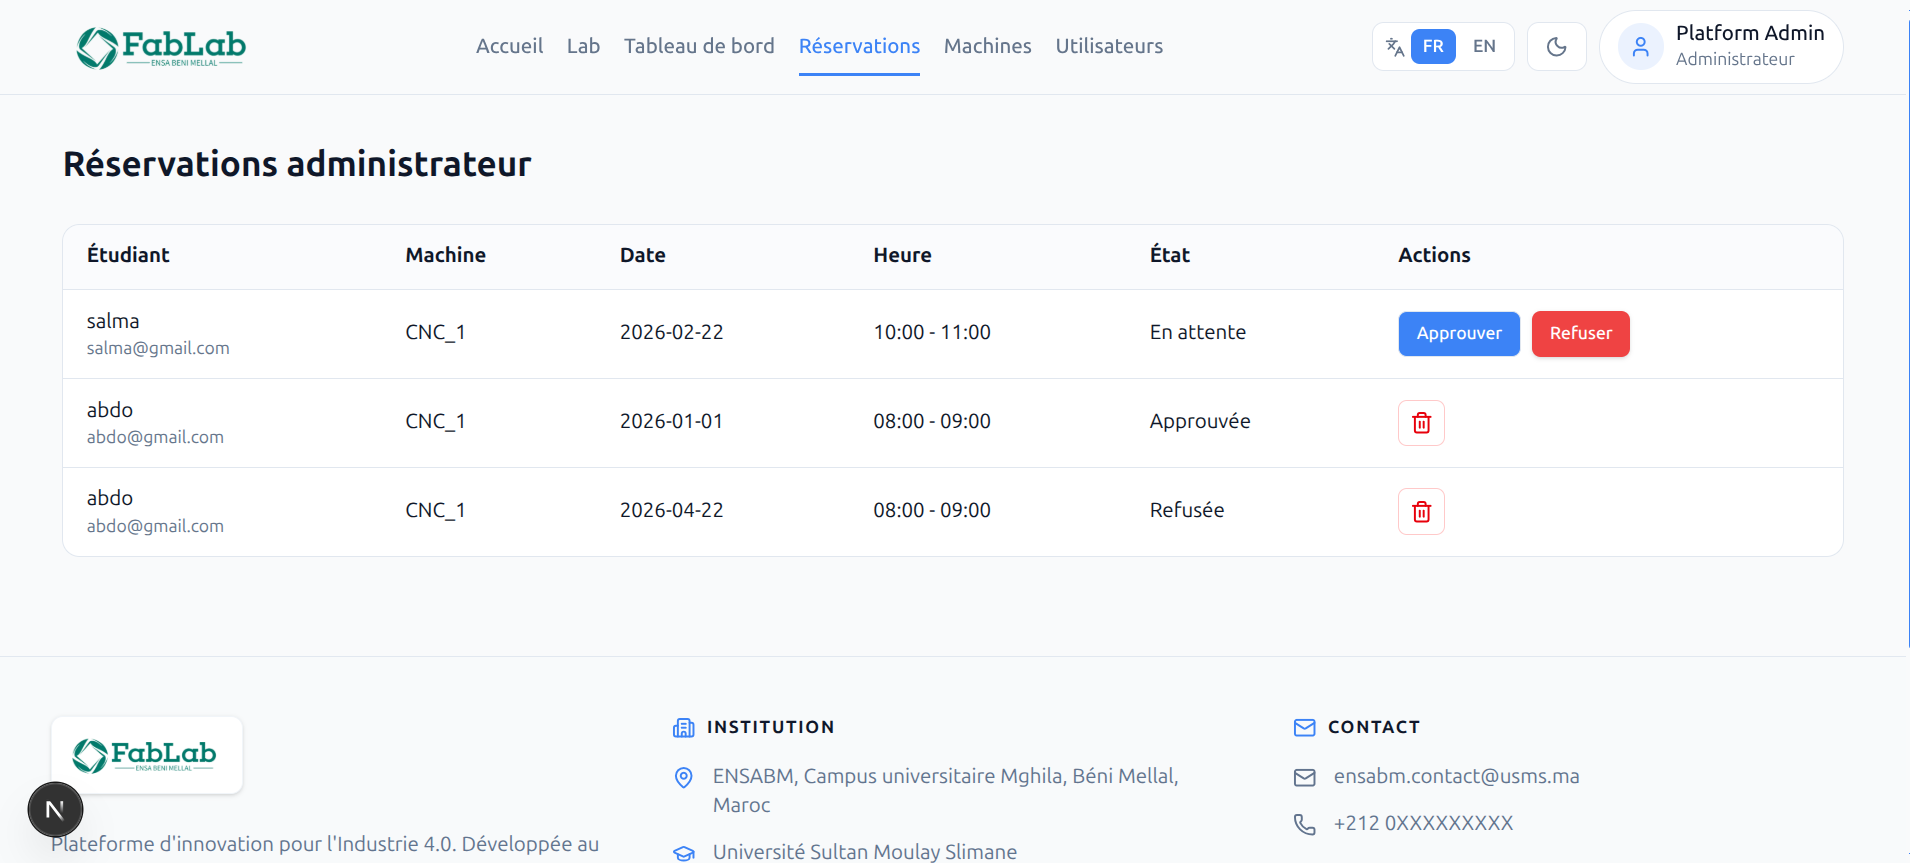
\includegraphics[width=0.95\textwidth]{images/screenshot_reservations.png}}
{\fbox{\parbox[c][5cm][c]{0.85\textwidth}{\centering Emplacement réservé pour l’interface de réservation\\\texttt{images/screenshot\_reservations.png}}}}
\caption{Interface de réservation des machines}
\label{fig:screenshot-reservations}
\end{figure}

\section{FabLab virtuel en 3D}

La page du laboratoire virtuel affiche une scène 3D représentant l’espace du FabLab. Les machines sont chargées dynamiquement depuis le backend, ce qui permet d’afficher les machines réellement enregistrées dans la base de données.

Chaque machine possède un modèle GLB, une position, une rotation et une échelle. L’utilisateur peut sélectionner une machine dans la scène afin de consulter son état, ses mesures récentes et ses actions disponibles : consulter les détails, ouvrir la simulation ou réserver.

\begin{figure}[H]
\centering
\IfFileExists{images/screenshot_lab_3d.png}
{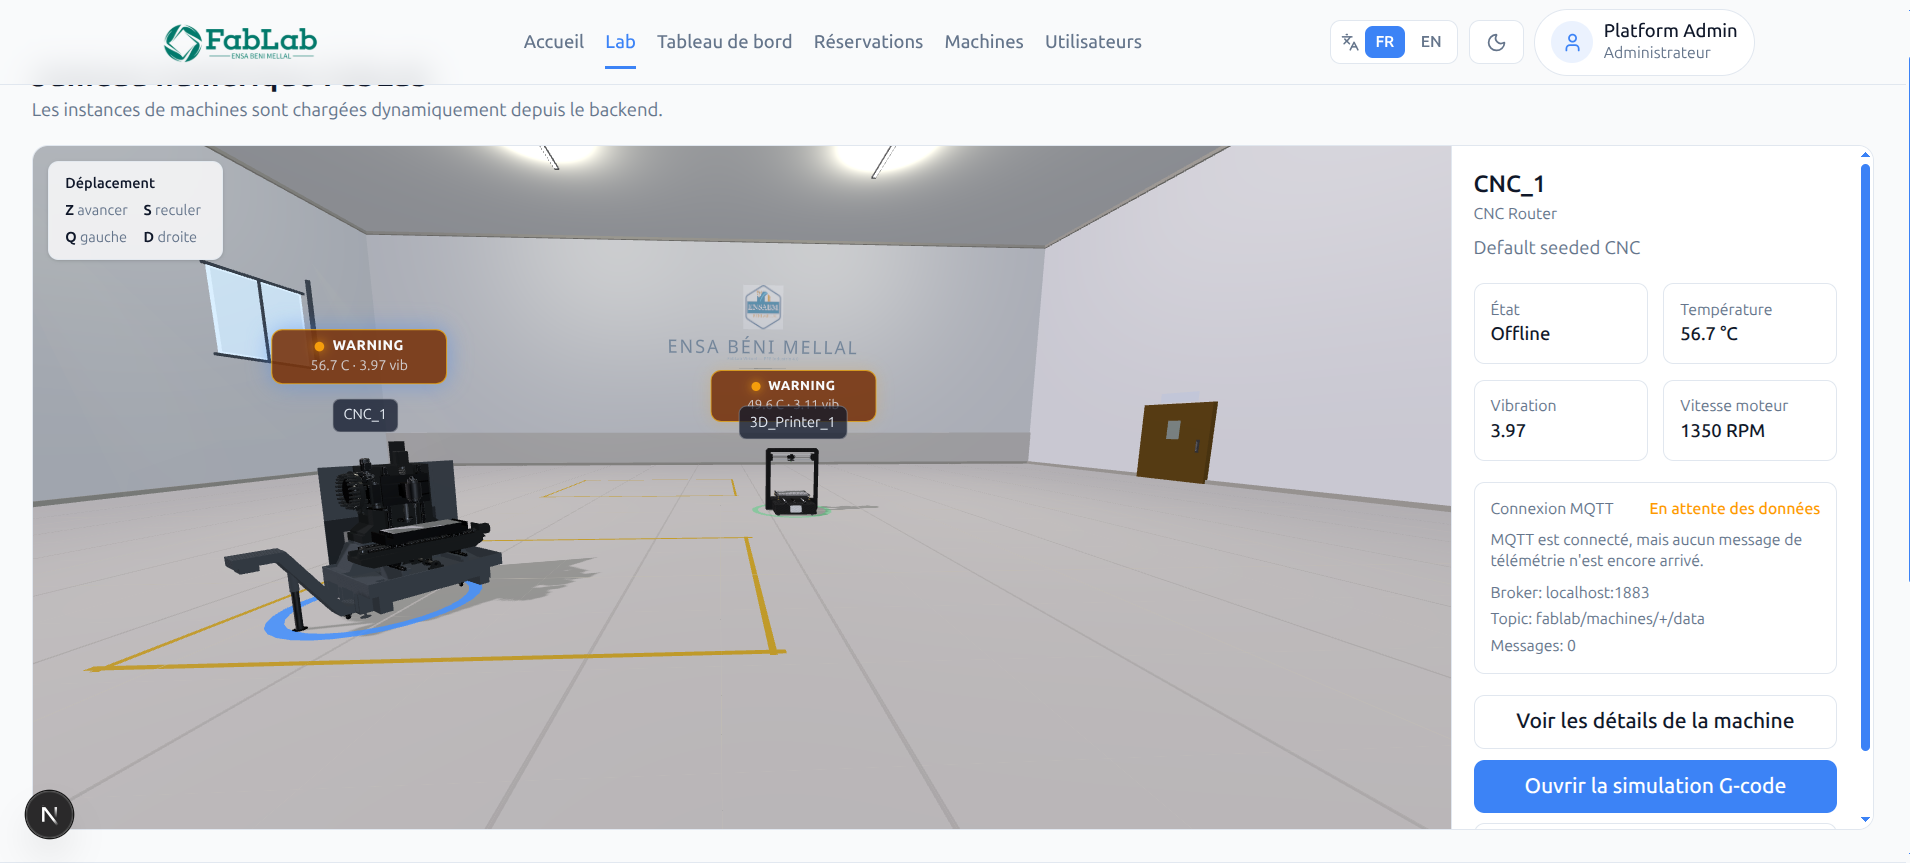
\includegraphics[width=0.95\textwidth]{images/screenshot_lab_3d.png}}
{\fbox{\parbox[c][5.5cm][c]{0.85\textwidth}{\centering Emplacement réservé pour la scène du FabLab virtuel\\\texttt{images/screenshot\_lab\_3d.png}}}}
\caption{Vue 3D du FabLab virtuel}
\label{fig:screenshot-lab-3d}
\end{figure}

\section{Simulation CNC}

La simulation CNC repose sur l’interprétation de fichiers NC ou G-code adaptés à une machine de fraisage ou de découpe. Le module détecte les commandes de mouvement, les vitesses d’avance, les arcs, les commandes de broche et certains signaux caractéristiques de la CNC.

Les trajectoires sont transformées en mouvements simulables dans la scène 3D. Les déplacements rapides et les opérations de coupe sont représentés différemment afin de distinguer les phases de positionnement et les phases d’usinage.

\begin{figure}[H]
\centering
\IfFileExists{images/screenshot_cnc_simulation.png}
{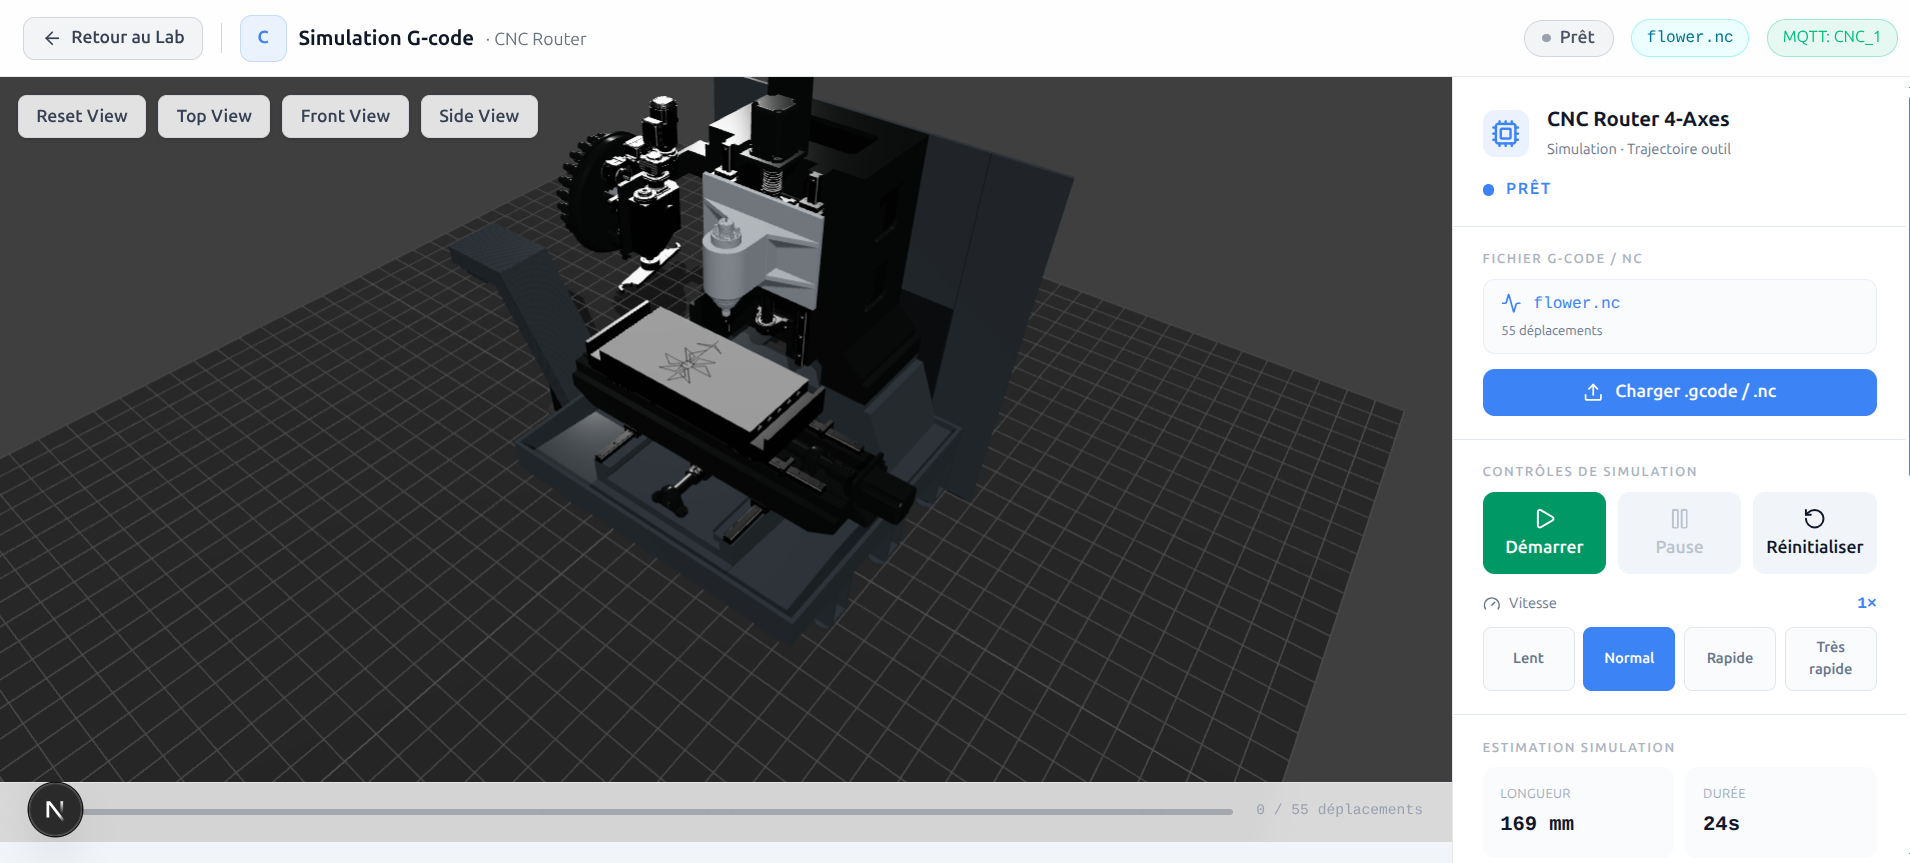
\includegraphics[width=0.95\textwidth]{images/screenshot_cnc_simulation.png}}
{\fbox{\parbox[c][5cm][c]{0.85\textwidth}{\centering Emplacement réservé pour la simulation CNC\\\texttt{images/screenshot\_cnc\_simulation.png}}}}
\caption{Simulation d’une trajectoire CNC}
\label{fig:screenshot-cnc-simulation}
\end{figure}

\section{Simulation de l’imprimante 3D}

La simulation de l’imprimante 3D prend en charge les fichiers G-code contenant les déplacements, l’axe d’extrusion, les vitesses d’avance et certaines commandes propres à l’impression 3D. Le système distingue les déplacements sans extrusion des segments imprimés.

La scène affiche progressivement la trajectoire d’impression et peut représenter les couches de l’objet. Le panneau latéral permet de suivre la progression, la position courante, la vitesse de lecture, la température simulée et les informations associées à la télémétrie lorsque la machine sélectionnée est liée à une instance enregistrée dans le backend.

\begin{figure}[H]
\centering
\IfFileExists{images/screenshot_printer_simulation.png}
{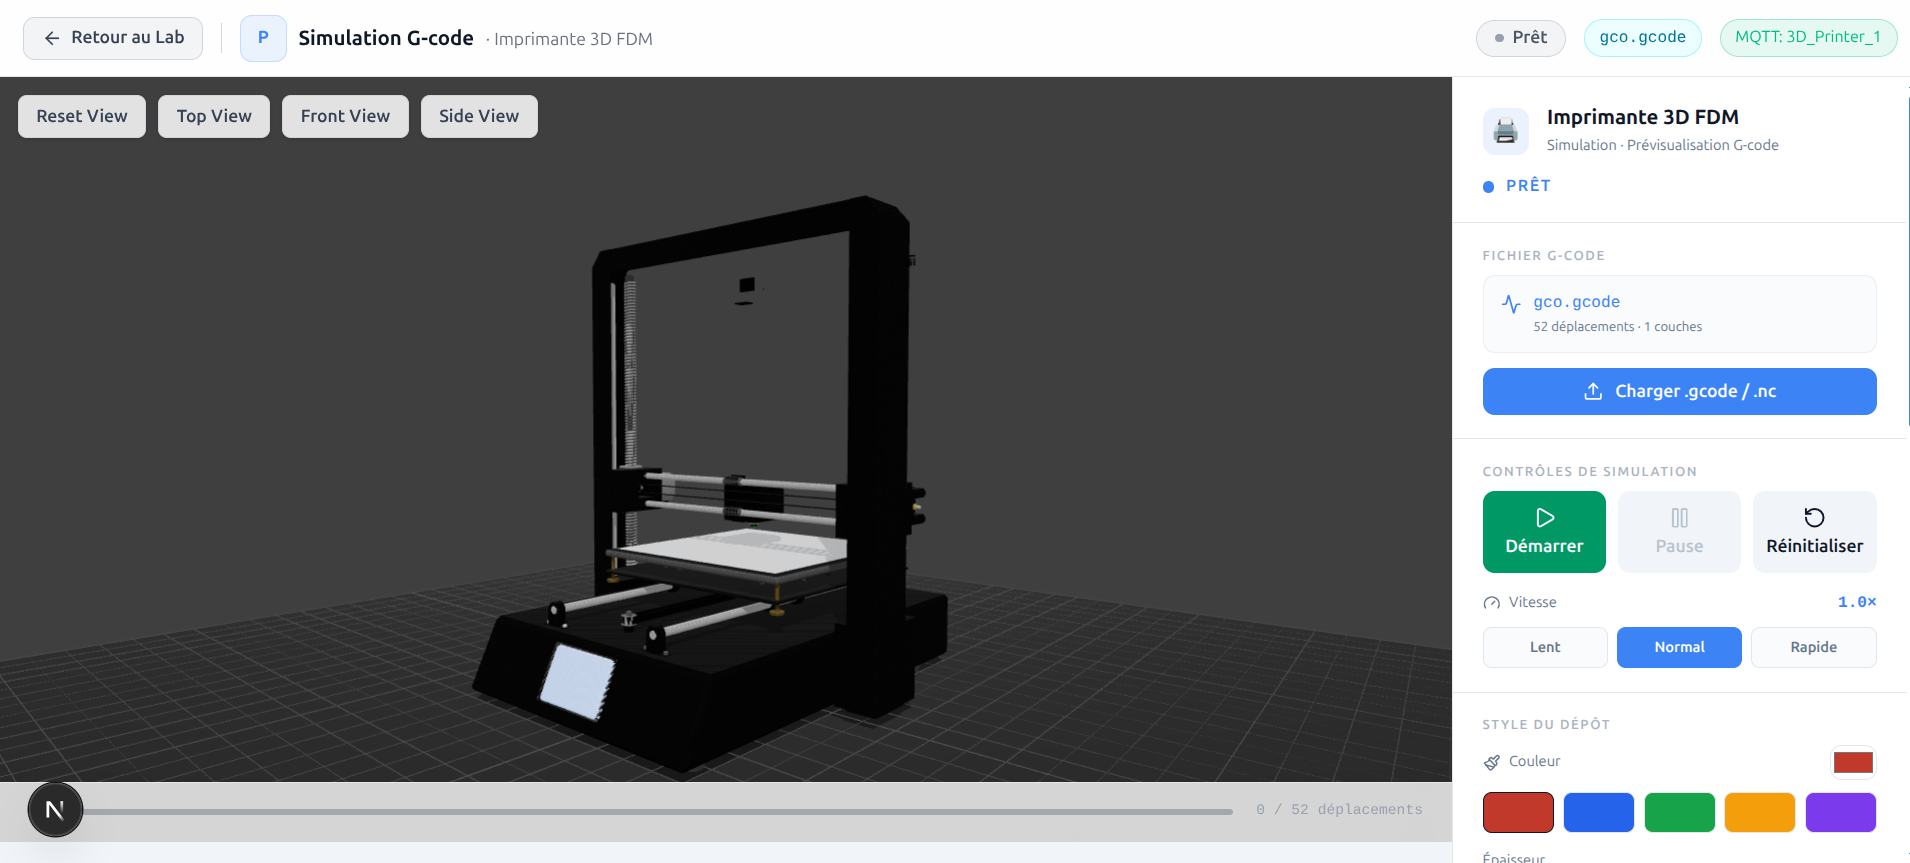
\includegraphics[width=0.95\textwidth]{images/screenshot_printer_simulation.png}}
{\fbox{\parbox[c][5cm][c]{0.85\textwidth}{\centering Emplacement réservé pour la simulation de l’imprimante 3D\\\texttt{images/screenshot\_printer\_simulation.png}}}}
\caption{Simulation d’un fichier G-code pour imprimante 3D}
\label{fig:screenshot-printer-simulation}
\end{figure}

\section{Interprétation des fichiers G-code et NC}

L’interprétation des fichiers est réalisée côté frontend afin de fournir un retour immédiat à l’utilisateur. Les lignes sont normalisées, les commentaires sont ignorés et les tokens de type \texttt{G}, \texttt{M}, \texttt{X}, \texttt{Y}, \texttt{Z}, \texttt{F}, \texttt{E}, \texttt{I}, \texttt{J} ou \texttt{R} sont analysés.

Le système vérifie également la compatibilité du fichier avec la machine sélectionnée. Par exemple, un fichier contenant des commandes de broche ou de refroidissement est considéré comme non compatible avec l’imprimante 3D, tandis qu’un fichier contenant des commandes d’extrusion est rejeté pour la CNC.

\begin{figure}[H]
\centering
\IfFileExists{images/gcode_validation_flow.png}
{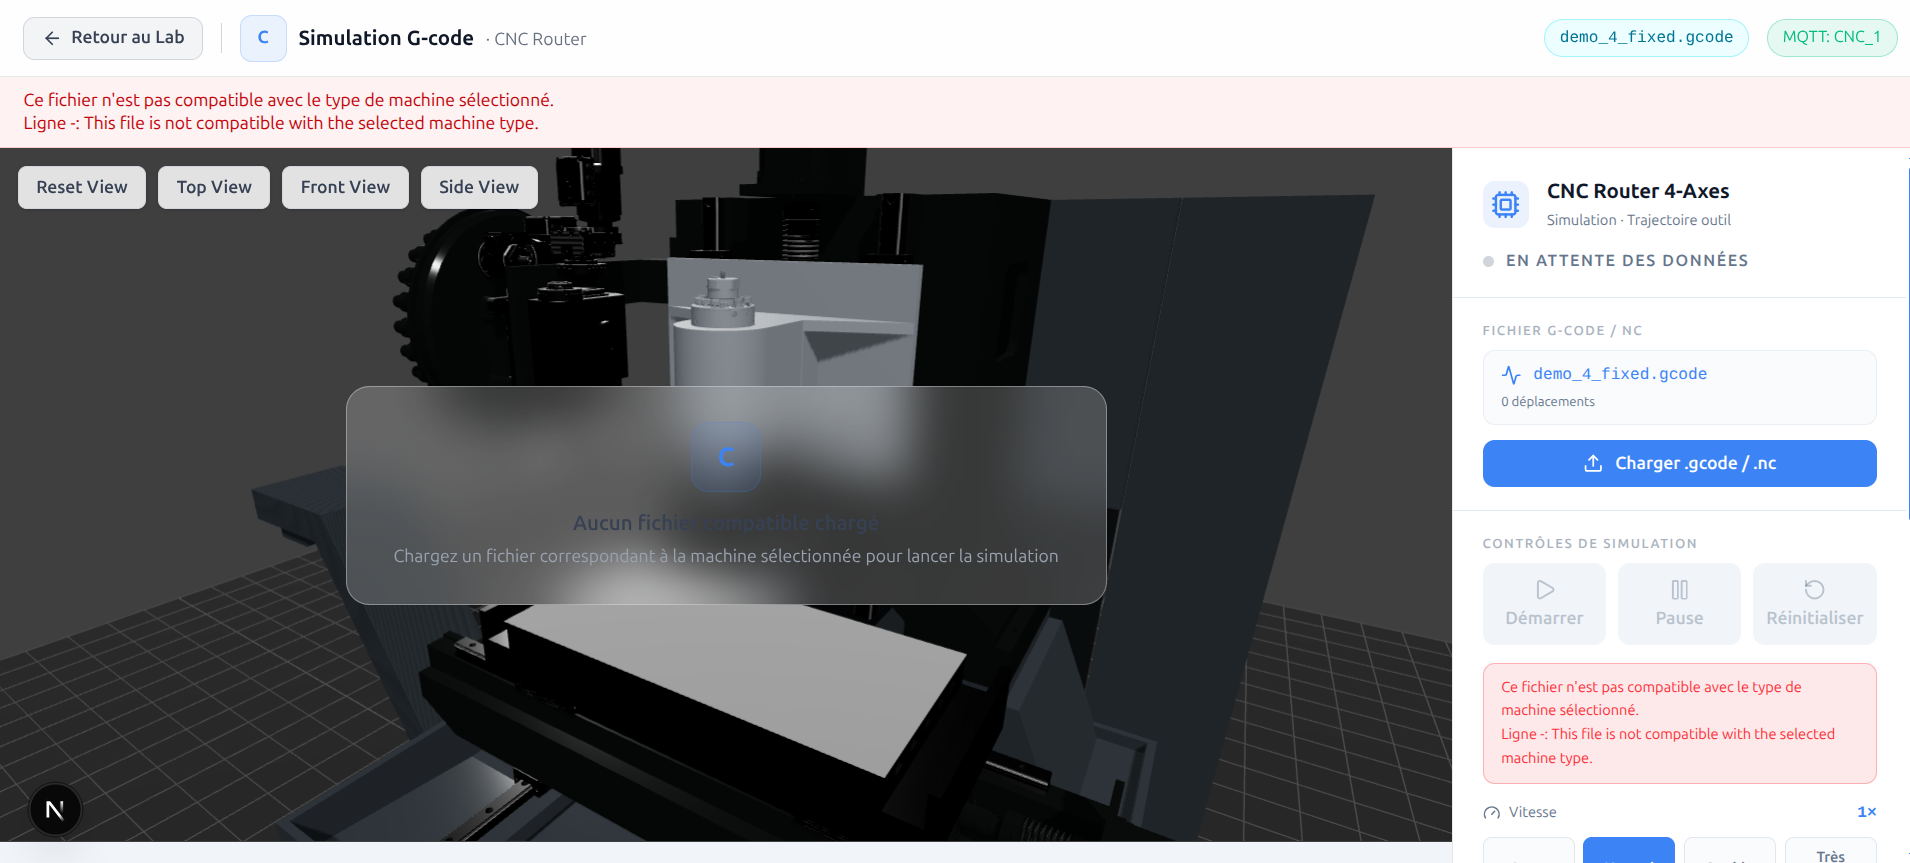
\includegraphics[width=0.9\textwidth]{images/gcode_validation_flow.png}}
{\fbox{\parbox[c][5cm][c]{0.85\textwidth}{\centering Emplacement réservé pour le processus d’interprétation G-code/NC\\\texttt{images/gcode\_validation\_flow.png}}}}
\caption{Processus d’interprétation et de validation des fichiers G-code/NC}
\label{fig:gcode-validation-flow}
\end{figure}

\section{Télémétrie simulée avec MQTT}

La télémétrie est simulée par un script Python qui publie périodiquement des messages MQTT. Ce choix permet de valider le flux complet sans dépendre, à ce stade, d’une installation physique de capteurs. Les données utilisées dans cette version sont simulées afin de valider l’architecture, les flux MQTT, le monitoring et le module d’analyse. La plateforme reste conçue pour être connectée ultérieurement à des capteurs réels. Chaque message est envoyé sur un topic de la forme :

\begin{center}
\texttt{fablab/machines/\{machine\_id\}/data}
\end{center}

Le message contient l’identifiant de la machine, la température, la vibration, la durée d’utilisation, la vitesse du moteur, une éventuelle erreur et un horodatage. Le backend s’abonne au motif \texttt{fablab/machines/+/data}, analyse les messages JSON et enregistre les mesures dans la base de données SQLite.

\begin{figure}[H]
\centering
\IfFileExists{images/mqtt_flow_real.png}
{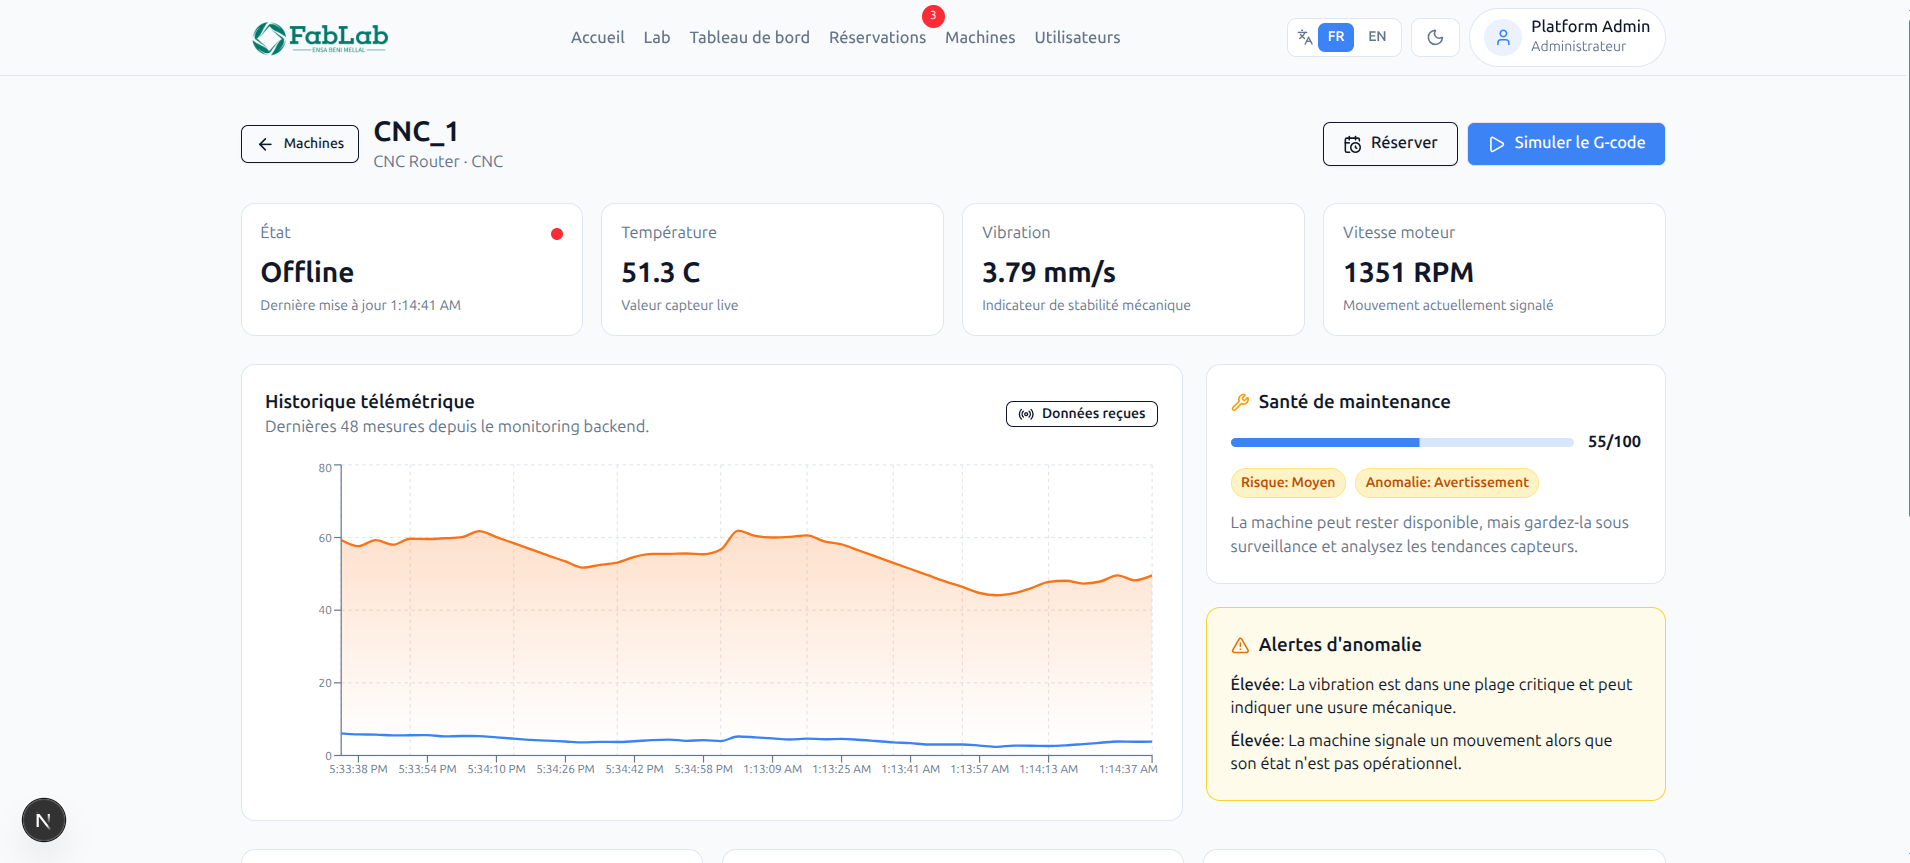
\includegraphics[width=0.95\textwidth]{images/mqtt_flow_real.png}}
{\fbox{\parbox[c][5cm][c]{0.85\textwidth}{\centering Emplacement réservé pour le flux MQTT implémenté\\\texttt{images/mqtt\_flow\_real.png}}}}
\caption{Flux MQTT implémenté dans la plateforme}
\label{fig:mqtt-flow-real}
\end{figure}

\section{Tableau de bord de supervision}

Le tableau de bord administrateur centralise les informations de supervision. Il affiche l’état de la connexion MQTT, la fraîcheur des données, le nombre d’utilisateurs, le nombre de machines, les réservations en attente et les résultats de monitoring intelligent.

Sur le plan de l’implémentation, le frontend interroge les endpoints administrateur du backend afin d’afficher les résultats calculés par les services d’analyse. Les éléments restitués incluent notamment :

\begin{itemize}
    \item un statut d’anomalie par machine ;
    \item un score de santé sur 100 ;
    \item un niveau de risque de maintenance ;
    \item une probabilité indicative de risque ;
    \item une recommandation de maintenance ;
    \item des facteurs explicatifs tels que température, vibration, durée d’utilisation, vitesse du moteur et erreurs récentes.
\end{itemize}

Les principes scientifiques, les caractéristiques utilisées, les modèles Machine Learning et les limites de validation sont détaillés dans le chapitre suivant afin d’éviter la duplication entre l’implémentation logicielle et la contribution analytique.

\begin{figure}[H]
\centering
\IfFileExists{images/screenshot_dashboard_ds.png}
{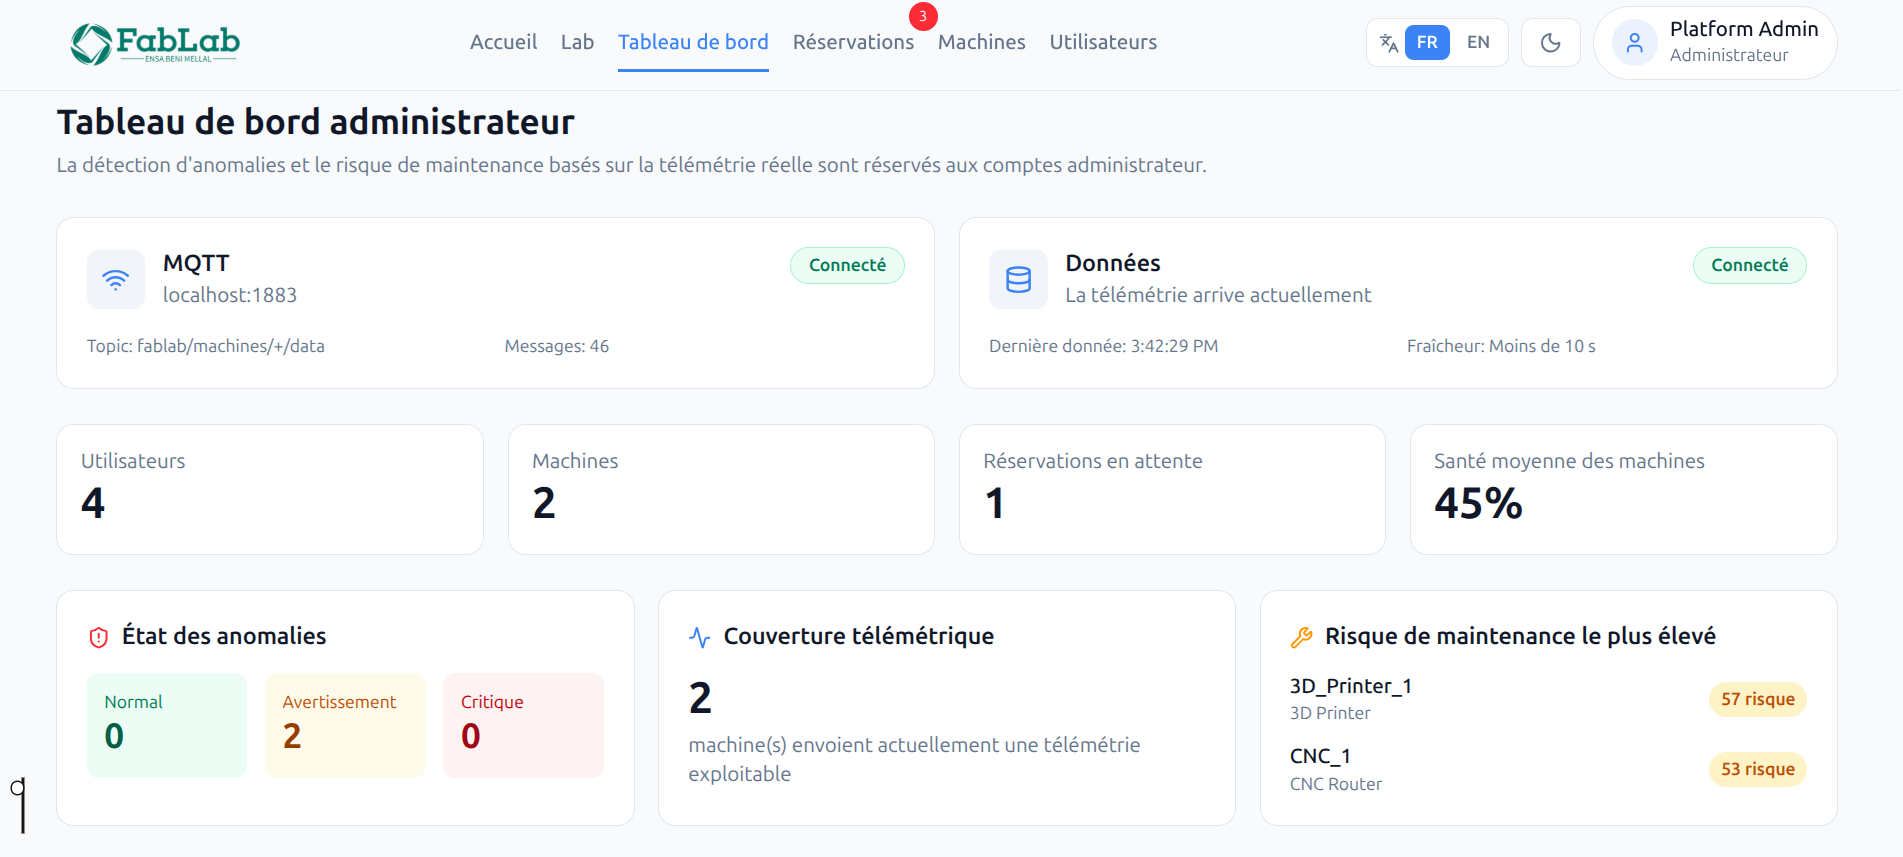
\includegraphics[width=0.95\textwidth]{images/screenshot_dashboard_ds.png}}
{\fbox{\parbox[c][5.5cm][c]{0.85\textwidth}{\centering Emplacement réservé pour le tableau de bord Data Science\\\texttt{images/screenshot\_dashboard\_ds.png}}}}
\caption{Tableau de bord administrateur et supervision intelligente}
\label{fig:screenshot-dashboard-ds}
\end{figure}

\section{Cartes de prédiction et historique de télémétrie}

Les cartes de prédiction du tableau de bord permettent de consulter rapidement les machines présentant un besoin de surveillance. Elles affichent les résultats déjà calculés par le backend : score de santé, probabilité indicative, niveau de risque et recommandation synthétique. Cette partie relève de l’intégration applicative, tandis que le détail des modèles est présenté séparément dans le chapitre consacré au module Data Science et IA.

\begin{figure}[H]
\centering
\IfFileExists{images/screenshot_prediction_cards.png}
{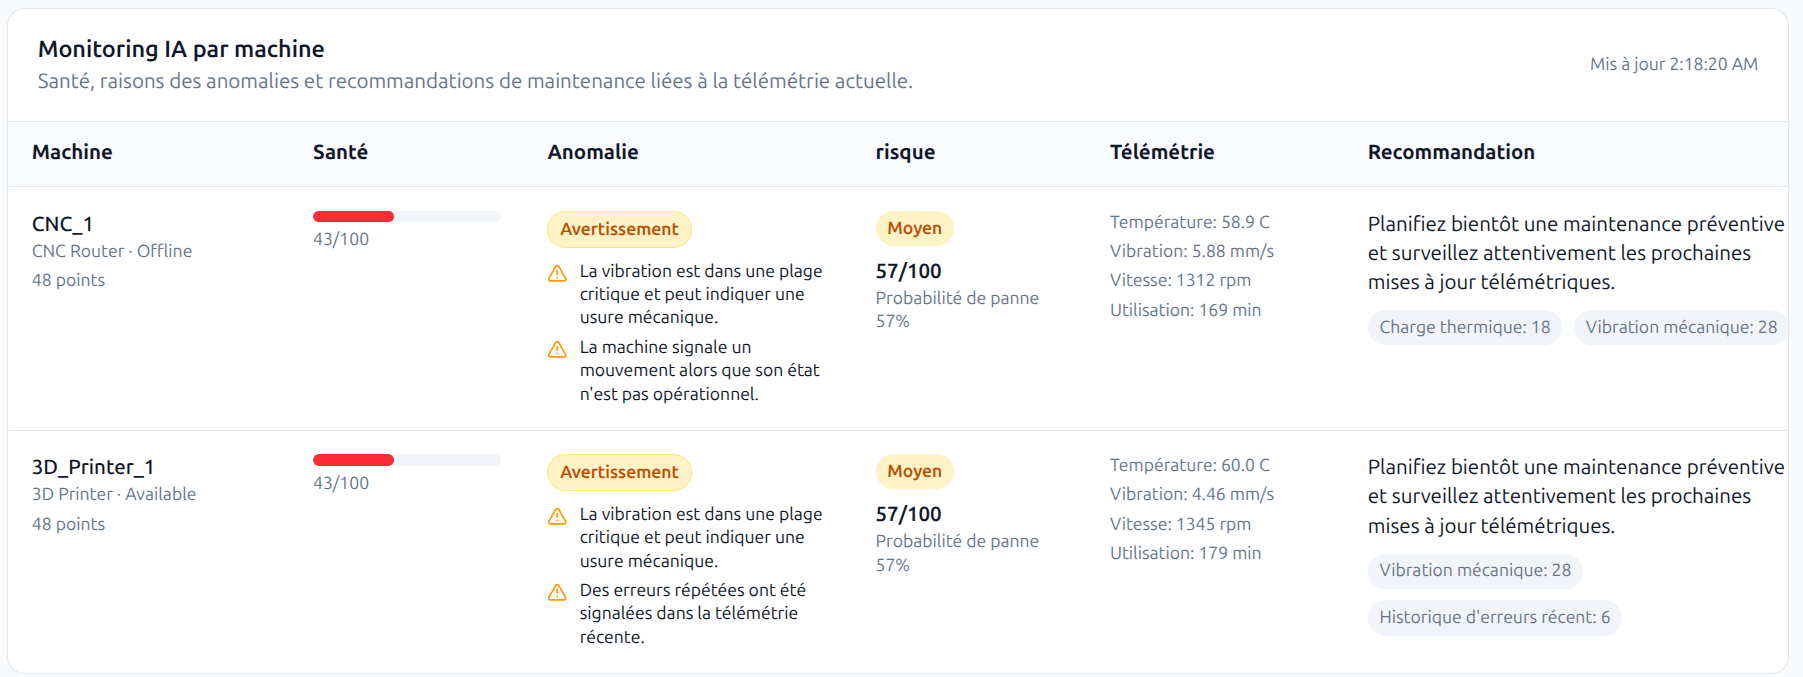
\includegraphics[width=0.95\textwidth]{images/screenshot_prediction_cards.png}}
{\fbox{\parbox[c][5cm][c]{0.85\textwidth}{\centering Emplacement réservé pour les cartes de prédiction\\\texttt{images/screenshot\_prediction\_cards.png}}}}
\caption{Cartes de prédiction et score de santé des machines}
\label{fig:screenshot-prediction-cards}
\end{figure}

Les pages de détail des machines exploitent l’historique des mesures stockées pour afficher l’évolution de certains indicateurs, notamment la température. Cette visualisation permet à l’administrateur de suivre l’état récent d’une machine et de relier les alertes à une série temporelle.

\begin{figure}[H]
\centering
\IfFileExists{images/screenshot_telemetry_history.png}
{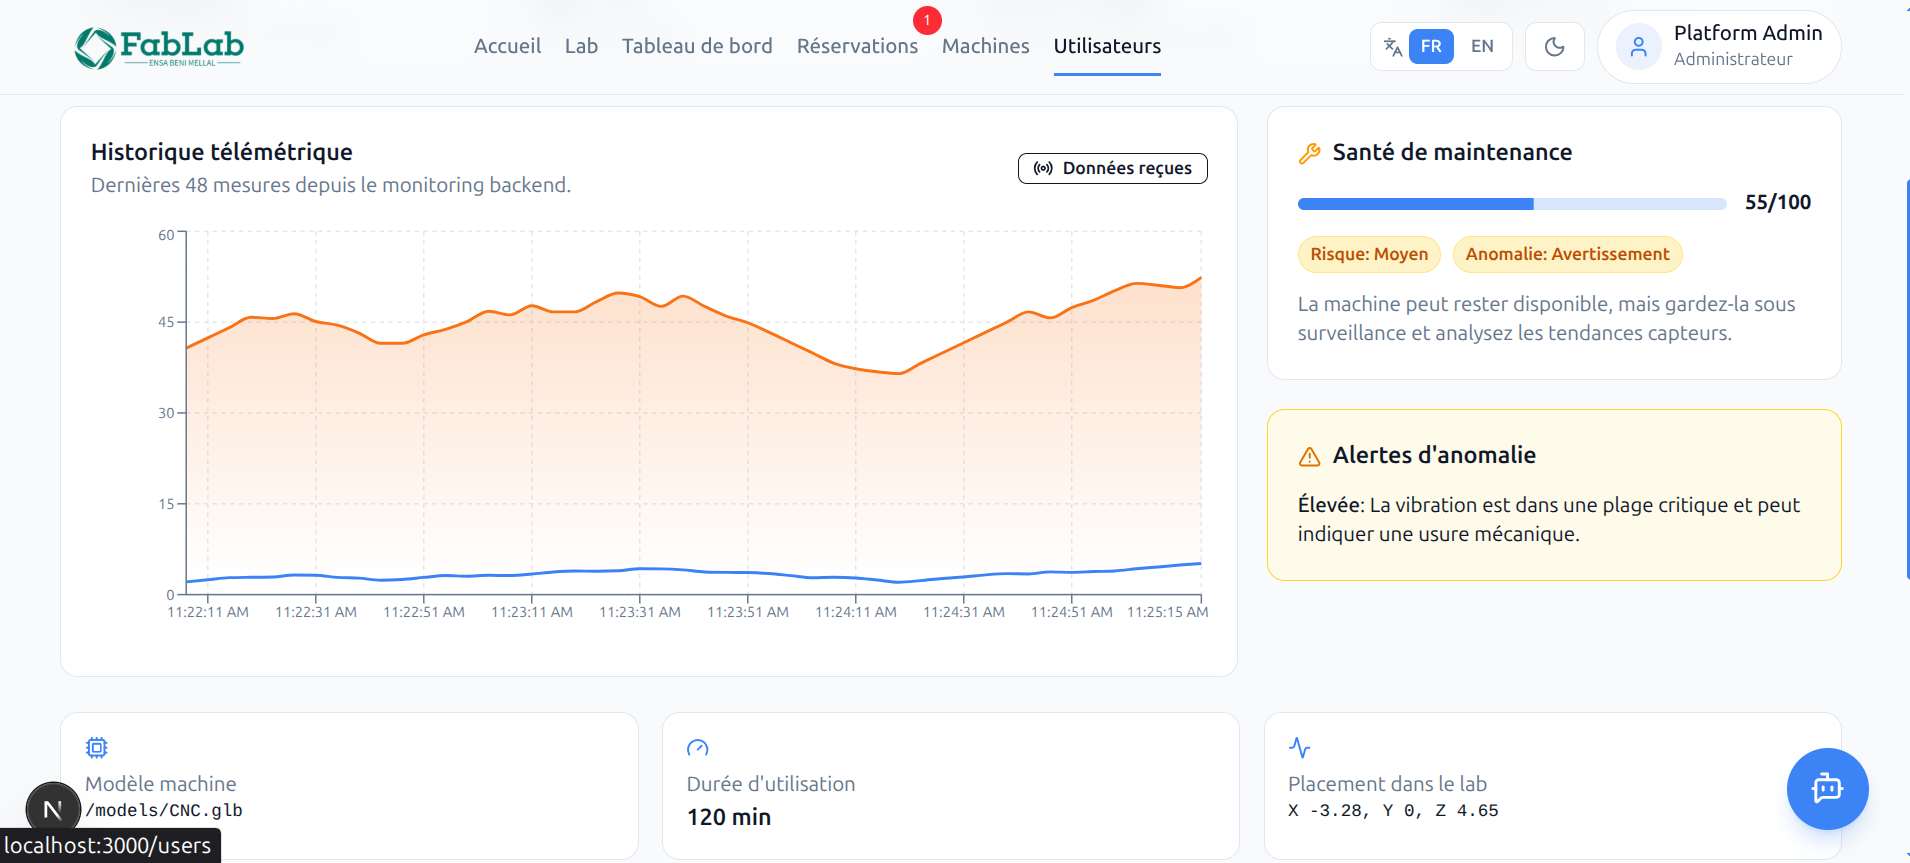
\includegraphics[width=0.95\textwidth]{images/screenshot_telemetry_history.png}}
{\fbox{\parbox[c][5cm][c]{0.85\textwidth}{\centering Emplacement réservé pour l’historique de télémétrie\\\texttt{images/screenshot\_telemetry\_history.png}}}}
\caption{Historique des mesures d’une machine}
\label{fig:screenshot-telemetry-history}
\end{figure}

\section{Intégration technique du Copilote IA}

L’espace administrateur intègre une interface flottante de type chatbot appelée Assistant IA de Maintenance. Cette interface est chargée dans le layout de l’application, mais elle n’est affichée que lorsque l’utilisateur connecté possède le rôle \texttt{admin}. Elle conserve l’historique de conversation localement dans l’état React du composant et envoie les questions au backend à travers l’endpoint \texttt{/admin/ai/copilot/query}.

Le frontend affiche la réponse structurée retournée par le backend : intention reconnue, niveau de sévérité, confiance, texte de synthèse, points de données et recommandations. Cette intégration fournit un accès conversationnel aux informations du tableau de bord, sans transformer le système en modèle génératif. Le fonctionnement scientifique du classifieur d’intentions et la génération déterministe des réponses sont détaillés dans le chapitre suivant.

\section{Communication entre frontend et backend}

La communication entre le frontend et le backend est centralisée dans une fonction utilitaire d’appel API. Cette fonction construit l’URL du backend, ajoute l’en-tête \texttt{Content-Type}, insère le jeton d’authentification lorsque nécessaire et traite les erreurs HTTP.

Cette couche simplifie l’usage des API dans les pages Next.js. Elle permet également de maintenir une cohérence dans la gestion des réponses, des erreurs et des routes protégées.

\begin{figure}[H]
\centering
\IfFileExists{images/api_communication.png}
{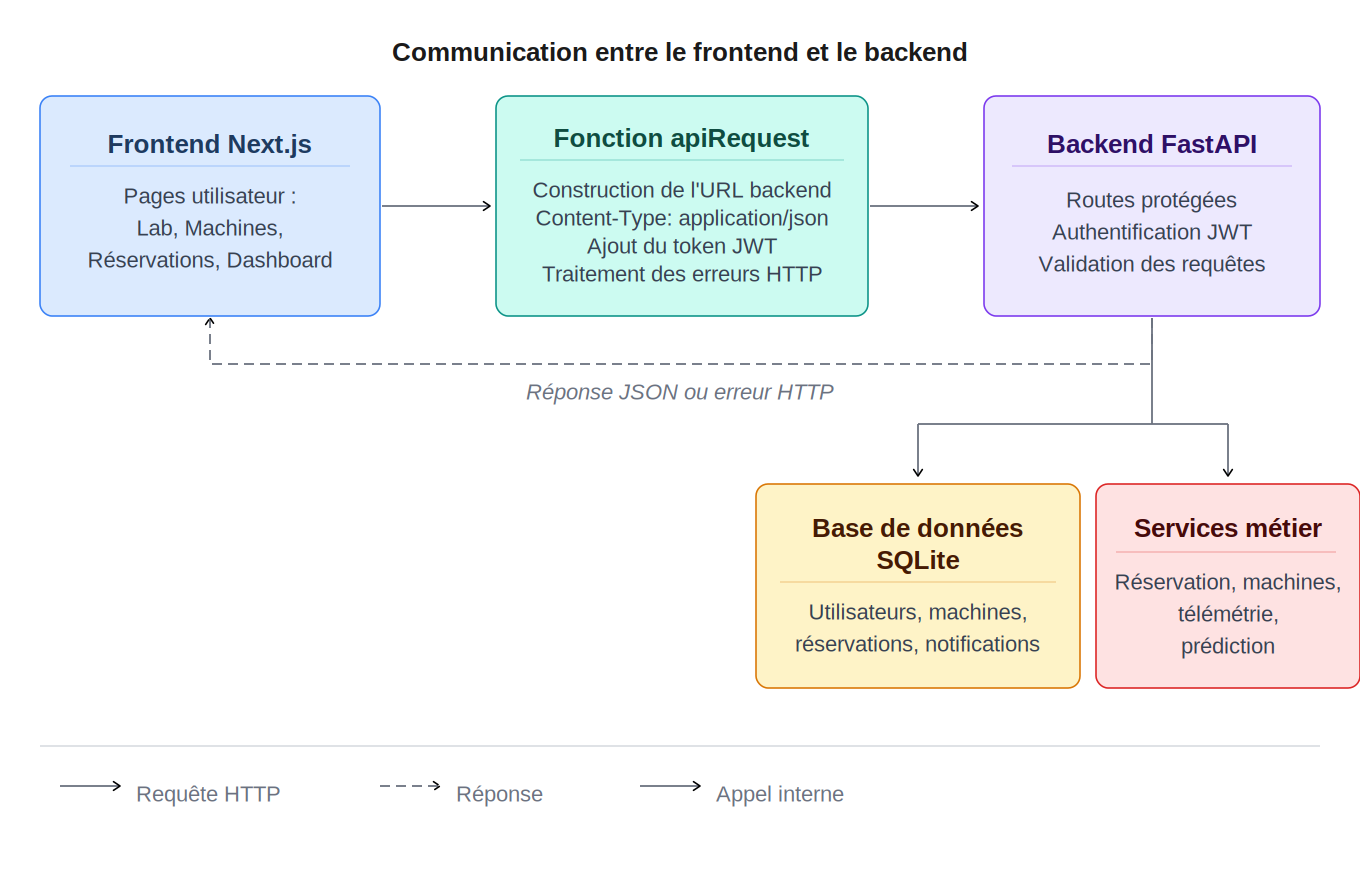
\includegraphics[width=0.9\textwidth]{images/api_communication.png}}
{\fbox{\parbox[c][5cm][c]{0.85\textwidth}{\centering Emplacement réservé pour le schéma de communication API\\\texttt{images/api\_communication.png}}}}
\caption{Communication entre le frontend et le backend}
\label{fig:api-communication}
\end{figure}

\section{Interfaces réalisées}

Les interfaces réalisées couvrent les principaux parcours utilisateurs : accueil, connexion, inscription, laboratoire 3D, simulation, réservation, profil, gestion des machines, gestion des utilisateurs, réservations administrateur et tableau de bord. Les captures présentées dans les sections précédentes illustrent les écrans les plus représentatifs de ces parcours.

\section{Conclusion}

Ce chapitre a présenté la réalisation technique de la plateforme Virtual FabLab. L’implémentation couvre la gestion des utilisateurs, des machines et des réservations, la visualisation du laboratoire en 3D, la simulation CNC et imprimante 3D, l’ingestion MQTT, le tableau de bord de supervision et l’intégration technique du Copilote IA.

Le chapitre suivant approfondira l’exploitation des données IoT et l’intégration de la Data Science et de l’IA, en détaillant les données utilisées, les modèles de détection, la classification d’intentions, les recommandations de maintenance et les limites de l’approche adoptée.
